\chapter{Introducción}
\label{chap:introducion}

% \lettrine{P}{rimer} capítulo da memoria, onde xeralmente se exporán as
% liñas mestras do traballo, os obxectivos, etc. Incluimos un par de
% exemplos de citas~\cite{ErlangBook,ErlangWebBook} e de referencias
% internas (sección \ref{sec:mostra}, páxina \pageref{sec:mostra}).

\lettrine{L}{a} vendimia es la recolección de la uva, que se procesa y se trata para obtener vino. 
Esta actividad milenaria se realiza normalmente en los meses de septiembre y octubre, cuando se recogen los frutos maduros de la vid.
Es un evento en el que se reúne mucha gente para "apañar" la uva, y motivo de festividad~\cite{Vendimia} en muchos puntos de Galicia(y del mundo).
Normalmente, en viñas domésticas no muy extensas, el trabajo es muy manual y no requiere de mucha gente y tiempo para la recolectar toda la uva.
Lo mas habitual es que hagan uso de un sistema de emparrado de conducción horizontal, l, típico en el rural gallego, especialmente en las Rías Baixas, 
donde las plantas de vids se forman con una estructura de pasillo de "arcos" ~\ref{fig:emparrado}. A pesar de su belleza en el rural, normalmente están construidos 
para la "comodidad" de cada dueño de la vid, por lo que puede ser difícil encontrar dos arcos a la misma altura. Esto hace que la recolección de la uva se mas difícil para personas de distinta altura 
y además dificulta el uso de maquinaria especifica como los tractores~\ref{fig:tractorEmparrado}.


  \begin{figure}[hp!]
    \centering
    \begin{subfigure}[c]{0.75\textwidth}
      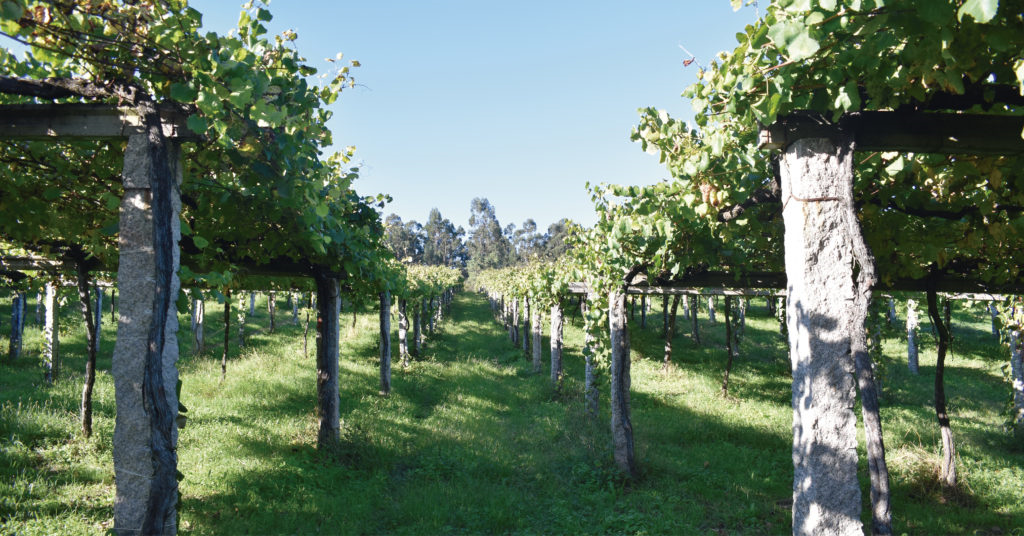
\includegraphics[width=\textwidth]{imaxes/sistema_emparrado.png}
      \caption{Formación vid emparrado}
      \label{fig:emparrado}
    \end{subfigure}
    \hspace{0.1\textwidth}
    \begin{subfigure}[c]{0.65\textwidth}
      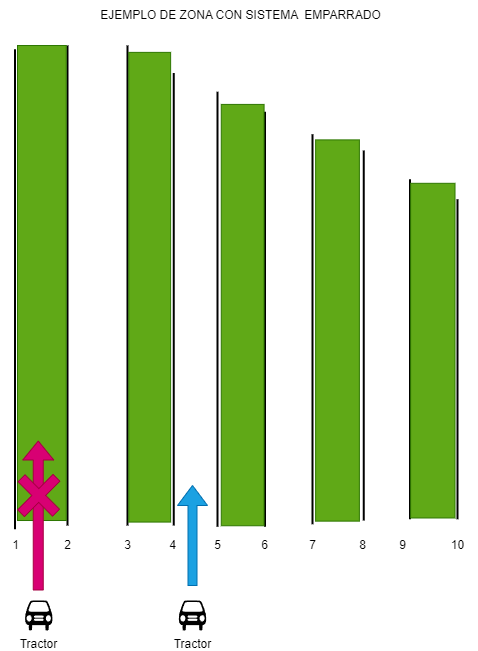
\includegraphics[width=\textwidth]{imaxes/2-EmparradoTractor.png}
      \caption{Maquinaria en emparrado}
      \label{fig:tractorEmparrado}
    \end{subfigure}
    \caption{Sistema de formación Emparrado}
    \label{fig:exemplo-subfiguras}
  \end{figure}
  
En empresas viticultoras con viñas extensas que recolectan muchas toneladas de uva, dependiendo del tamaño del terreno utilizado para el cultivo de las vides, 
el tipo de uva y su rendimiento ~\cite{RendimientoViticultura}.A pesar de que muchas empresas siguen teniendo vides en formación de emparrado horizontal, aprovechando así vides antiguas para la producción de vino de mayor calidad, 
se suele utilizar una formación de parras verticales, denominada formación espaldera ~\ref{fig:espaldera}. Esta formación en espaldera es mucho mas eficiente para trabajar, 
tanto para operarios de mantenimiento en tareas como podas, control de plagas y enfermedades, y el uso de maquinaria para tareas fitosanitarias, como para operarios de la vendimia, ya que la recolección es mucho mas sencilla 
y facilita el uso de maquinaria para la recogida de las cajas de uvas.~\ref{fig:tractorEspaldera}


\begin{figure}[hp!]
    \centering
    \begin{subfigure}[c]{0.75\textwidth}
      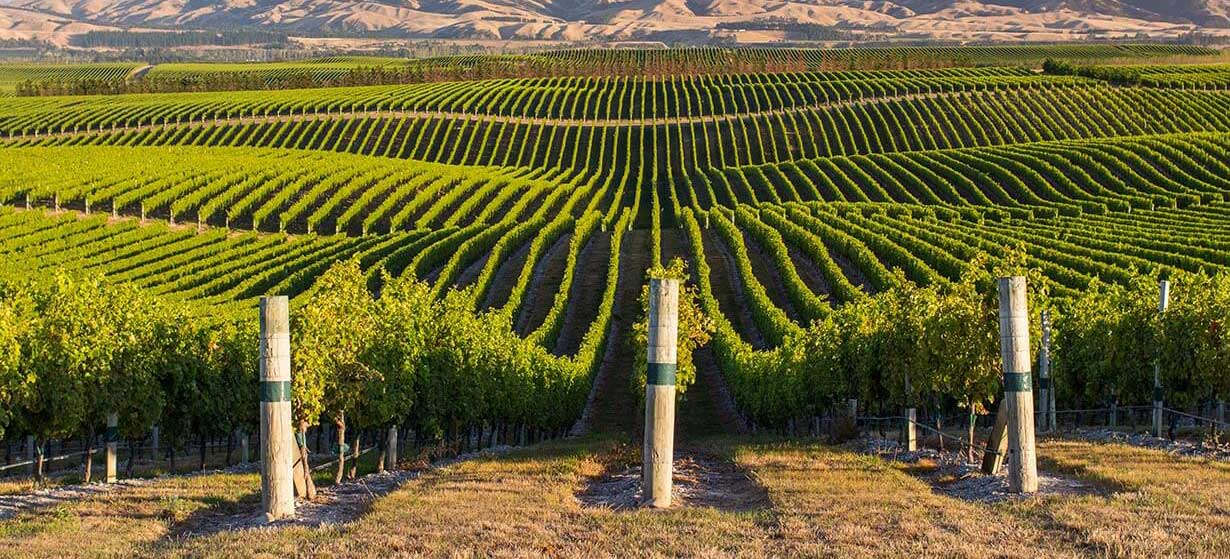
\includegraphics[width=\textwidth]{imaxes/3-Espalderas.png}
      \caption{Formación vid emparrado}
      \label{fig:espaldera}
    \end{subfigure}
    \hspace{0.1\textwidth}
    \begin{subfigure}[c]{0.65\textwidth}
      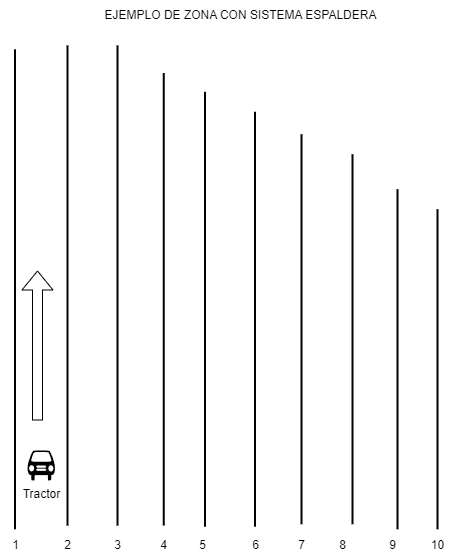
\includegraphics[width=\textwidth]{imaxes/4-EspalderasTractor.png}
      \caption{Maquinaria en emparrado}
      \label{fig:tractorEspaldera}
    \end{subfigure}
    \caption{Sistema de formación Espaldera}
    \label{fig:exemplo-subfiguras}
  \end{figure}


  Cada año en una empresa viticultora realiza una campaña para la vendimia. Esta campaña consiste en la ejecución de tareas específicas en todas las líneas de vides. 
  En concreto, el grupo de tareas esenciales en cada linea para la realización de una vendimia son las siguientes:
\begin{description}
  \item[Limpieza de las líneas:] Consiste principalmente en la limpieza de los pasillos entre dos lineas de vides para facilitar las siguientes tareas. 
  Normalmente, la tarea consiste en desbrozar, y suele ser personal propio de la empresa viticultora quien realiza esta tarea.

  \item[Poda de las líneas:] Consiste en podar las hojas y ramas que estorban y que pueden entorpecer el trabajo de la recolección. 
  En estas tareas trabajan conjuntamente capataces y personal de vendimia (personal externo) con experiencia previa.
  
  \item[Recolección de la uva:]
  La tarea más significativa para la vendimia. Consiste en el corte de los racimos de uva y su almacenamiento en cajas, 
  Estas cajas se llenan y se almacenan debajo de la estructura de la linea de la vid para facilitar la siguiente tarea de carga. 
  En estas tareas, solo el personal de vendimia trabajara en las líneas, mientras que los empleados de la empresa supervisan el trabajo realizado 
  (por lo que a partir de aquí denominare capataces a los empleados de las vids). Estas son las más criticas y demanda muchos recursos. 

  \item[Carga de las cajas de uva:] Durante esta tarea, un capataz con permiso de conducción de tractor, junto con, normalmente, tres personas más de personal de vendimia, 
  almacenarán las cajas de racimos de uva en el tractor, y cada vez que se llena el tractor o no queden cajas por recoger este será destinado a bodega donde se almacenaran los racimos de uva. Debe realizarse justo después de la recolección de la uva


\end{description}

\section{Motivación}

Durante el inicio de la campaña anual de la vendimia, comenzando con las tareas de limpieza, la empresa no necesita muchos cambios en la organización, ya que el propio personal de la empresa 
que realiza estas tareas. Sin embargo, a medida que avanza la campaña se incorpora mas gente, alcanzando el máximo en la tarea de recolección de la uva, 
por lo que la situación se vuelve caótica casi de un día para otro.
Durante la etapa de recolección pueden ocurrir numerosos incidentes que provoquen la pausa en la recogida de la uva, como climatología adversa que afecte a todas las líneas. 
Sin embargo, incidentes específicos en líneas individuales, como lesiones de los operarios, picaduras de avispas, golpes de calor o fatiga que impida la finalización de los trabajos asignados, también son situaciones comunes.
Evidentemente, los capataces atienden y socorren a los operarios de recolección en este tipo de situaciones. Sin embargo, después de atender a los operarios, 
a menudo pueden ocurrir desorganizaciones, como que el capataz  no recuerde la linea donde no se finalizo la recolección, cambios incorrectos en los turnos de capataces 
que resultan en confusión sobre qué líneas supervisar, o que los propios capataces enfrenten urgencias personales que los obliguen a abandonar su puesto.

Normalmente, el administrador gestiona el avance de la campaña de vendimia comunicándose con los capataces mediante llamadas y aplicaciones de mensajería instantánea.
Sin embargo, pueden ocurrir incidencias no notificadas que pueden llevar a una mala organización de los recursos y a un seguimiento deficiente del progreso de los trabajos en las lineas.

Por tanto, la creación de una aplicación móvil para ayudar en la organización de las tareas y en el control del progreso de las lineas seria beneficiosa. Esto facilitaría la coordinación tanto para los capataces como para los administradores.


\section{Objetivos}

Los principales objetivos con la realización del proyecto son, poner orden al caos con:
\begin{enumerate}
  \item Gestión de la información relativa a las lineas de vides, agrupadas por zonas. El administrador se encargara de decidir que lineas de vides son validas para su posterior recolección.
  \item Gestión de la los empleados de la empresa viticultora(capataces). El administrador se encarga de añadir a los capataces en el sistema, los cuales podrán hacer uso de la aplicación.
  \item Gestión de los operarios de vendimia. El administrador también es responsable de llevar un registro de la disponibilidad horaria de los operarios de vendimia, dado que puede variar considerablemente día a día. 
  Además, la aplicación permitirá tomar asistencia del personal de vendimia para eliminar su presencia del calendario en caso de ausencia ese mismo día, o incluso dar de baja de manera permanente.
  \item Gestión de las tareas de las líneas. Los capataces y los tractoristas son responsables de registrar el inicio de las tareas y de asignar los operarios de vendimia. 
  Además, serán ellos quienes registren la finalización de las tareas, incluyendo el porcentaje de avance y cualquier incidente ocurrido, permitiendo así un seguimiento completo de la vendimia.
  \item Idear funcionalidades que agilicen todo lo posible el proceso de seguimiento de las tareas.
\end{enumerate}

Además de los puntos anteriores, mis objetivos también son mejorar mis conocimientos de Spring Framework, iniciarme en el desarrollo de aplicaciones móviles con Flutter 
y documentarme y experimentar con la generación automática de código y documentación mediante el uso de la especificación OpenAPI.



% \Blindtext

% \section{Sección de mostra}
% \label{sec:mostra}

% \Blindtext

% \subsection{Subsección de mostra}

% \Blindtext
